\documentclass[11pt,a4paper]{article}
\usepackage[margin=2.3cm]{geometry}
\usepackage{graphicx}
\usepackage{booktabs}
\usepackage{xcolor}
\usepackage[colorlinks=true,linkcolor=blue!55!black,urlcolor=blue!55!black]{hyperref}
\usepackage{caption}
\usepackage{subcaption}
\captionsetup{font=small,labelfont=bf}
\graphicspath{{perf_results/}}
\setlength{\parskip}{0.5em}
\setlength{\parindent}{0pt}

\title{\textbf{Section 1, Question 1}\\[0.3em]
       \large Matrix Multiplication with MapReduce}
\author{Distributed Systems --- Homework 3}
\date{}

\begin{document}
\maketitle
\vspace{-2.5em}

\section{What the question asks}

Multiply two matrices, $A$ of size $m \times n$ and $B$ of size $n \times p$,
using the MapReduce programming model: independent map tasks running on separate
machines, a shuffle that groups related values together, and a reduce step that
produces the final matrix.

The implementation must handle arbitrary matrix shapes, including cases where
the number of rows does not divide evenly by the number of tasks, and must
produce the same answer regardless of how many tasks are used.

\section{How the multiplication is decomposed}

To compute one output cell $C[i][j]$ you need row $i$ of $A$ and column $j$ of
$B$. The decomposition rests on a simple observation: if a map task is given
\textbf{whole rows of $A$} and can read \textbf{all of $B$}, then it can compute
every cell in its own rows without consulting any other task. That independence
is what makes the work splittable.

\begin{description}
\item[Map.] For each row $i$ of $A$ held by this task, and each column $j$ of
  $B$, emit \texttt{i,j <TAB> partial value}.
\item[Combine.] A task usually produces several partials for the same cell. The
  combiner adds them locally, so less data crosses the network.
\item[Shuffle.] \texttt{sort -k1,1} places all values for one cell together. No
  program performs the shuffle --- the sort is the shuffle.
\item[Reduce.] Walk the sorted stream, sum the values sharing a key, print the
  finished matrix.
\end{description}

The pipeline is therefore five stages: split $A$ by rows, map, sort per machine,
combine, sort globally, reduce. Splitting by rows is what permits any task
count: a task that receives no rows simply produces nothing, which is why a
matrix with $1001$ rows divided among four tasks works exactly as well as one
with $1000$.

\section{What was implemented}

\begin{center}\small
\begin{tabular}{@{}llr@{}}
\toprule
\textbf{File} & \textbf{Role} & \textbf{Lines} \\
\midrule
\texttt{mapper.py} & emits one partial product per output cell & 45 \\
\texttt{combiner.py} & sums a task's own partials before they travel & 30 \\
\texttt{reducer.py} & sums partials per cell and prints the matrix & 40 \\
\texttt{verify.py} & multiplies directly, with no MapReduce --- the oracle & 35 \\
\texttt{run\_cluster\_test.sh} & Slurm: the nine correctness cases & \\
\texttt{benchmark\_dist\_slurm.sh} & Slurm: seven matrix shapes at four machines & \\
\texttt{benchmark\_scaling\_slurm.sh} & Slurm: three sizes $\times$ 1, 2, 4, 7 machines & \\
\bottomrule
\end{tabular}
\end{center}

Everything is Python 3, which the compute nodes already provide, so there is no
build step.

\section{Correctness}

Nine cases, all passing, run distributed across four machines. Each result is
compared against \texttt{verify.py}, which performs the multiplication directly.

The cases are chosen so that each could plausibly fail for a different reason:
the assignment's worked example; a square matrix whose rows divide evenly by the
task count and one that does not ($1001$ rows over four tasks); a tall matrix
($5000 \times 10$); a wide one ($10 \times 500$), where most tasks receive
almost nothing; and the degenerate single-row and single-column cases.

The scaling benchmark adds a stronger check: \textbf{all $36$ of its runs} were
compared against the single-task answer, confirming that dividing the input
differently never changes the result.

\section{Results}

\subsection{Scaling: the larger the input, the better it scales}

Median of three runs, one map task per machine.

\begin{center}\small
\begin{tabular}{@{}lrrrrr@{}}
\toprule
\textbf{Input} & \textbf{1 machine} & \textbf{2} & \textbf{4} & \textbf{7} &
\textbf{Speedup at 7} \\
\midrule
Small ($100 \times 50$)   & 0.414\,s & 0.353\,s & 0.355\,s & 0.326\,s & $1.27\times$ \\
Medium ($500 \times 50$)  & 1.141\,s & 0.720\,s & 0.529\,s & 0.446\,s & $2.56\times$ \\
Large ($2000 \times 50$)  & 3.801\,s & 2.140\,s & 1.274\,s & 0.918\,s & $\mathbf{4.14\times}$ \\
\bottomrule
\end{tabular}
\end{center}

The pattern is the finding. Large reaches $4.14\times$ on seven machines
($59\%$ efficiency), Medium $2.56\times$ ($37\%$), and Small barely moves at
$1.27\times$ ($18\%$).

Every run carries a fixed cost that does not shrink when machines are added:
starting a Python interpreter on each node, reading all of $B$ on every task,
and five stages of process startup. On a $100 \times 50$ matrix there is so
little real work that this fixed cost is most of the runtime, so the extra
machines have almost nothing to divide.

The practical conclusion is that \textbf{small inputs should not be
distributed}. One machine finishes sooner than seven once coordination is
counted. This is the same conclusion Section~2 reaches for a completely
different workload, which suggests it is a property of the model rather than of
either program.

\begin{figure}[htbp]
\centering
\begin{subfigure}{0.49\textwidth}
  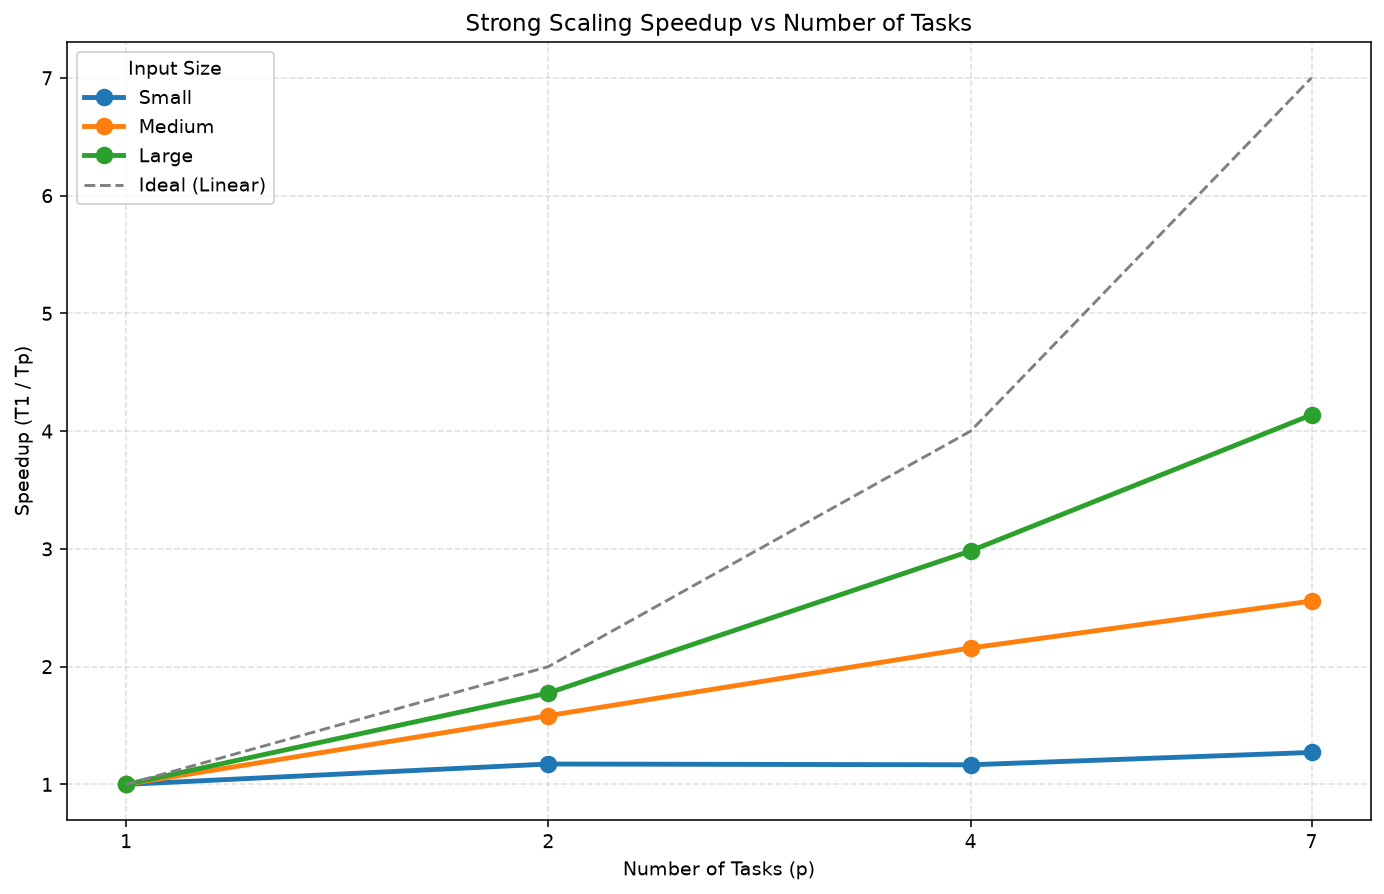
\includegraphics[width=\textwidth]{speedup.png}
\end{subfigure}
\hfill
\begin{subfigure}{0.49\textwidth}
  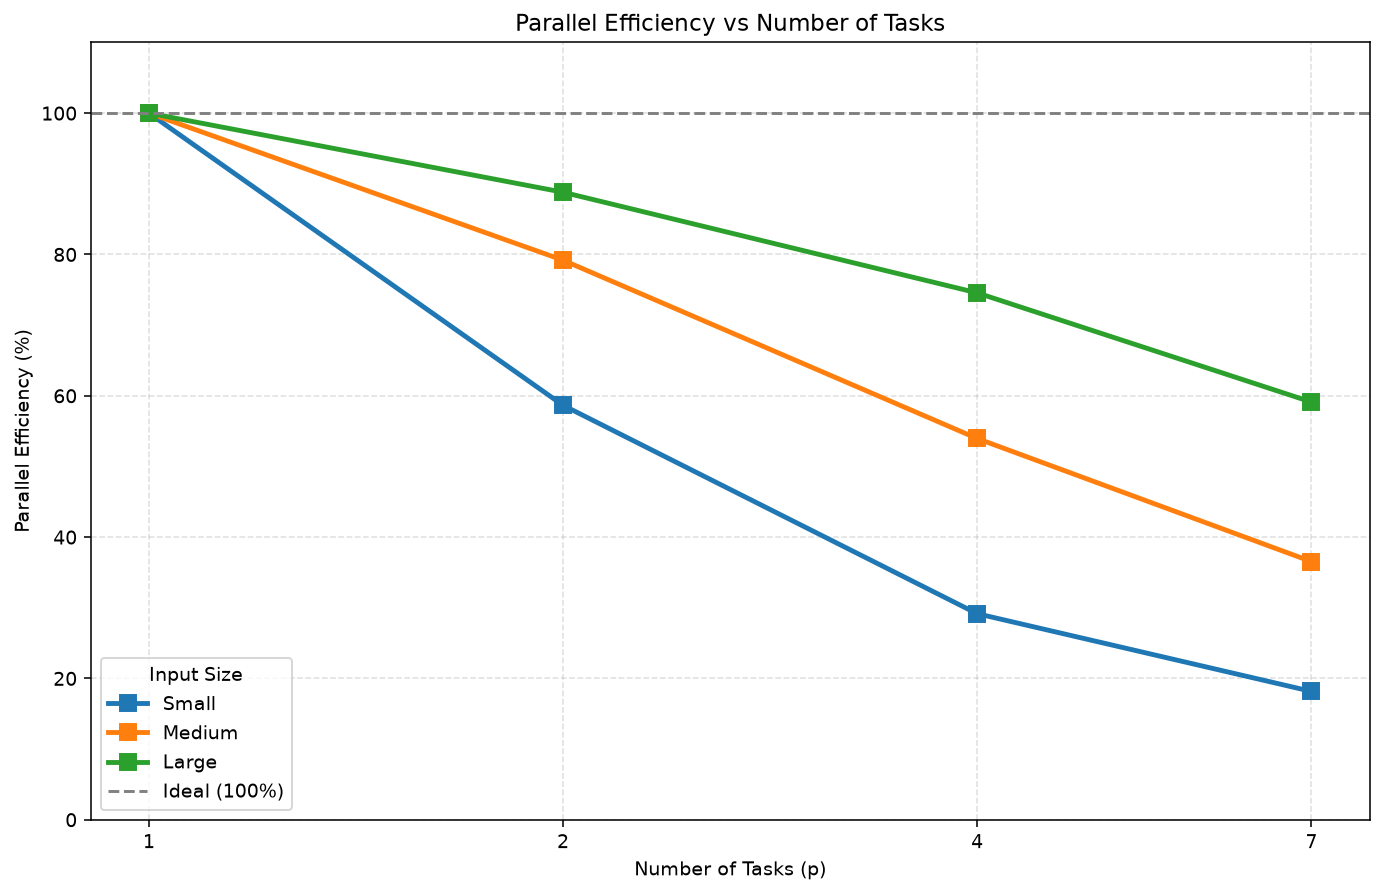
\includegraphics[width=\textwidth]{efficiency.png}
\end{subfigure}
\caption{Strong scaling. Left: speedup against the linear ideal --- the three
input sizes separate clearly, and only Large stays near the ideal. Right: the
same data as parallel efficiency, which falls for every size but far faster for
the small inputs.}
\end{figure}

\subsection{Shape matters more than size}

Seven matrix shapes, all on four machines.

\begin{center}\small
\begin{tabular}{@{}llrrrr@{}}
\toprule
\textbf{Shape} & \textbf{$A$} & \textbf{$B$} & \textbf{Map} & \textbf{Shuffle} & \textbf{Total} \\
\midrule
wide          & $10 \times 500$   & $500 \times 10$   & \phantom{0}0.22 & \phantom{0}0.19 & \phantom{0}0.65\,s \\
small         & $100 \times 50$   & $50 \times 50$    & \phantom{0}0.26 & \phantom{0}0.20 & \phantom{0}0.71\,s \\
tall          & $5000 \times 10$  & $10 \times 10$    & \phantom{0}0.34 & \phantom{0}0.24 & \phantom{0}0.93\,s \\
medium        & $500 \times 50$   & $50 \times 50$    & \phantom{0}0.45 & \phantom{0}0.23 & \phantom{0}1.07\,s \\
large         & $2000 \times 50$  & $50 \times 50$    & \phantom{0}1.15 & \phantom{0}0.42 & \phantom{0}2.45\,s \\
\textbf{square} & $1000 \times 100$ & $100 \times 1000$ & 17.53 & 20.55 & \textbf{50.22\,s} \\
square uneven & $1001 \times 100$ & $100 \times 1000$ & 18.34 & 22.99 & 53.96\,s \\
\bottomrule
\end{tabular}
\end{center}

\textbf{Square is twenty times slower than large}, despite having half as many
rows. The reason is the number of output cells: \texttt{large} produces
$2000 \times 50 = 100{,}000$ of them, while \texttt{square} produces
$1000 \times 1000 = 1{,}000{,}000$, and each requires $100$ partial products.
The cost follows $m \times n \times p$, not the size of $A$ --- so the row count,
which is what determines how the work is split, is a poor predictor of how long
a run will take.

\textbf{The shuffle becomes the bottleneck at scale.} For \texttt{square},
sorting takes $20.5$\,s of the $50.2$\,s total --- more than the mapping itself.
For every other shape it is under half a second. This is the characteristic
weakness of MapReduce: intermediate data must be materialised and sorted, and
that cost grows with the number of distinct keys, which here is the number of
output cells.

\textbf{Uneven splits cost very little.} $1001$ rows over four tasks takes
$53.96$\,s against $50.22$\,s for $1000$ rows. The single extra row lands on one
machine and the other three wait at the barrier --- a $7\%$ penalty, which is the
expected behaviour of a synchronisation point rather than a defect.

\begin{figure}[htbp]
\centering
\begin{subfigure}{0.49\textwidth}
  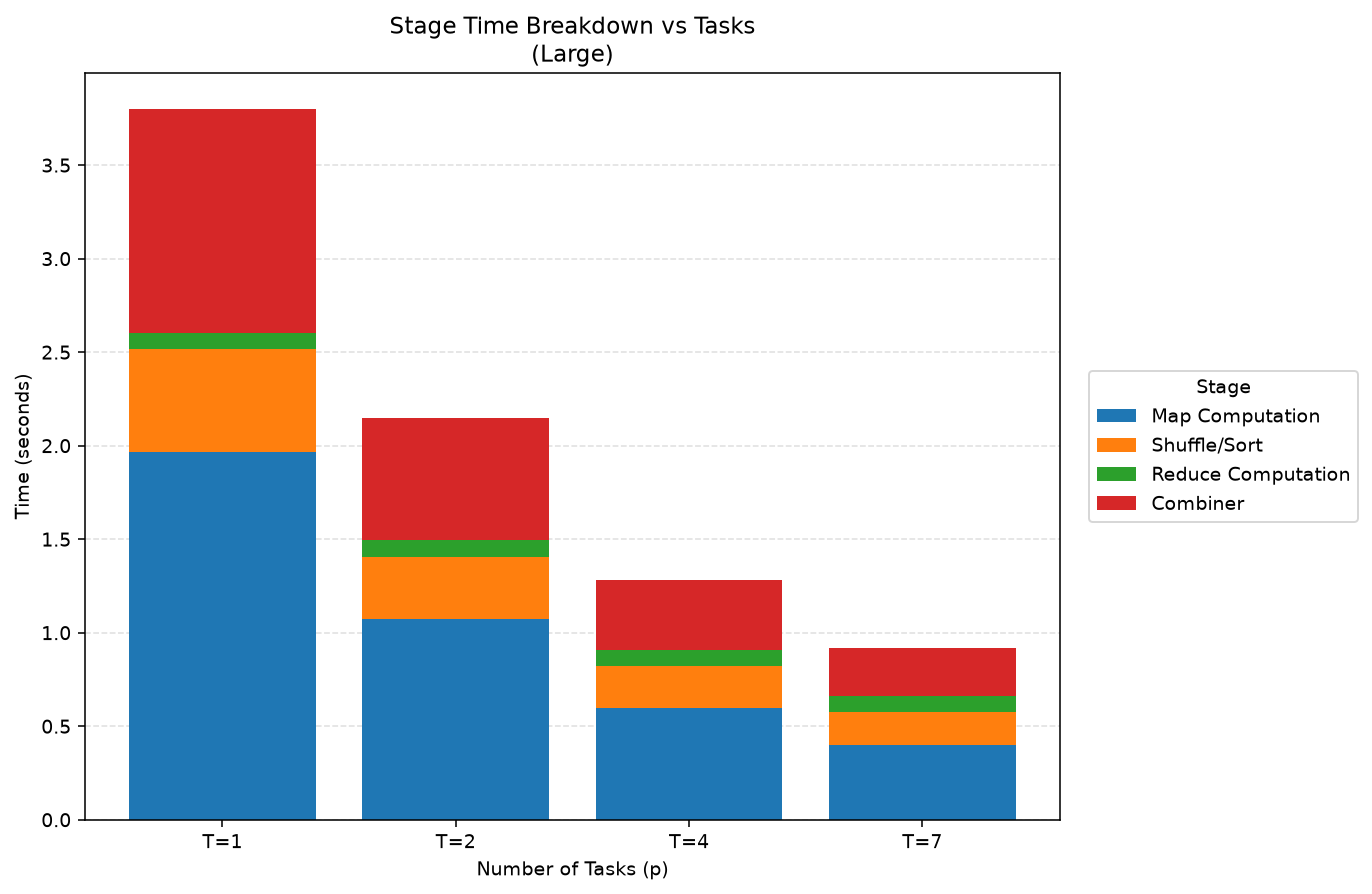
\includegraphics[width=\textwidth]{stages_Large.png}
\end{subfigure}
\hfill
\begin{subfigure}{0.49\textwidth}
  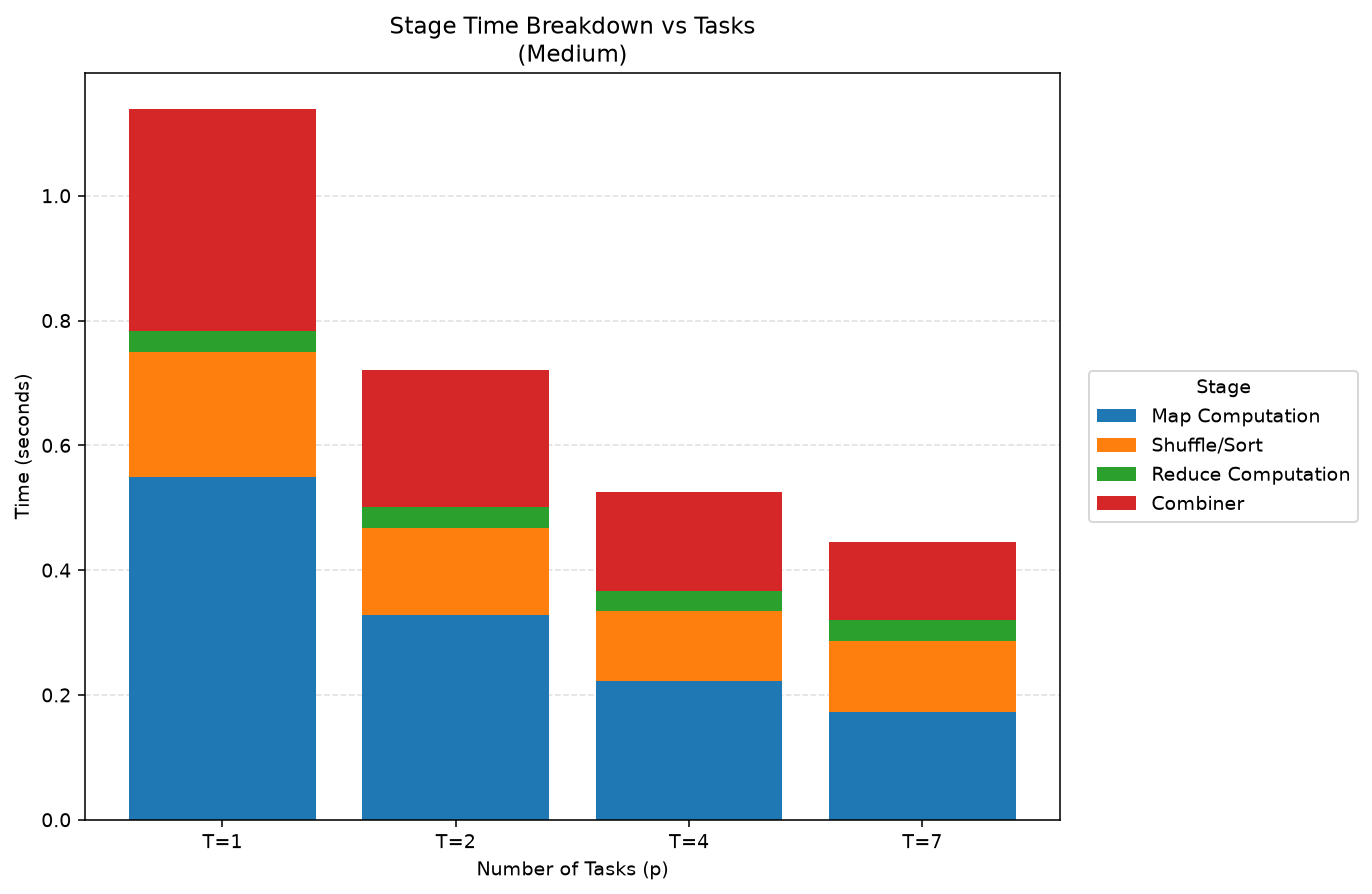
\includegraphics[width=\textwidth]{stages_Medium.png}
\end{subfigure}
\caption{Where the time is spent, for the Large and Medium inputs. The map stage
shrinks as machines are added, while the shuffle and the single reduce do not,
which is what limits the achievable speedup.}
\end{figure}

\section{A measurement trap worth recording}

Only seven of the cluster's eight nodes are usable. An earlier sweep nonetheless
requested eight map tasks. The allocation grants one task slot per machine, so
\texttt{srun --ntasks=8} across seven machines quietly started only \emph{seven}
tasks: one chunk of $A$ was never mapped.

The pipeline then produced a \textbf{wrong answer faster than the correct one} ---
$0.308$\,s at the nominal eight tasks against $0.327$\,s at four. A missing
chunk is indistinguishable from a speedup if only the clock is read.

Two changes followed. The sweep now runs 1, 2, 4 and 7 tasks, every point
strictly one task per machine; and the benchmark verifies that the number of map
outputs equals the number of chunks, stopping if they differ. The lesson
generalises: a performance result that is not accompanied by a correctness check
is not a result.

\section{Conclusions}

Matrix multiplication decomposes cleanly into MapReduce because each map task
can compute whole rows of the answer independently, given all of $B$. The
implementation is correct across all nine test cases and across every task
count tried.

Speedup depends strongly on having enough work to divide: $4.14\times$ on seven
machines for the largest input, but only $1.27\times$ for the smallest, where
fixed coordination costs dominate. Shape matters more than size, because cost
follows the number of output cells rather than the number of rows --- and for the
squarest case the shuffle, not the computation, becomes the limiting stage.
\end{document}
